\documentclass[UTF8]{ctexbook}

\usepackage{color}
\usepackage{amsmath}
\usepackage{amsthm}
\usepackage{amssymb}
\usepackage{tikz}
\usepackage{tikz-cd}


\author{李文威}
\date{\today}
\title{代数学方法-基础架构}

\theoremstyle{definition} \newtheorem{Def}{定义}[section]
\newtheorem{Them}{定理}[section]
\newtheorem{Prop}{命题}[section]
\newtheorem{Exap}{例}[section]
\newtheorem{Lem}{引理}[section]
\newtheorem{Coly}{Corollary}[section]
\newtheorem{Rmk}{注意}
\newtheorem{Sym}{符号}[section]
\newtheorem{Axm}{公理}[section]
\newtheorem{Asum}{假设}[section]
\newtheorem{Cvs}{约定}

\newcommand{\Obj}{\operatorname{Ob}}	% Objects
\newcommand{\Mor}{\operatorname{Mor}}   % Morphisms
\newcommand{\Hom}{\operatorname{Hom}}   % Homorphisms
\newcommand{\Isom}{\operatorname{Isom}} % Isomorphisms
\newcommand{\End}{\operatorname{End}}   
\newcommand{\Aut}{\operatorname{Aut}}
\newcommand{\identity}{\ensuremath{\mathrm{id}}}
\newcommand{\cate}[1]{\ensuremath{\mathsf{#1}}}	% Font series for categories

\begin{document}

    \maketitle

    \newpage
    
    \section[1]{Introductory ideas}
The definitions will be refer to all book, but 1.8 is refered to only in Section 3.5.

\textbf{Throughout the book, mapping symbols are written on the right.}

\subsection[1]{Basic definitions}

\begin{Def}[Semigroup]
    A groupoid $(S,\mu), S \neq \emptyset, \mu$ is a map $: S\times S \to S$ and $\mu$ is associative
    \begin{equation}
        \forall x,y,z \in S, ((x,y)\mu,z)\mu (x,(y,z)\mu)\mu
    \end{equation}
\end{Def}

The notation of operator $\mu$ could be notated as multiplication.

$$(x y)z=x(y z)$$

When the multiplication of semigroup is clear from the context, we shall write simply $S$ rather that $(S,.)$

\begin{Def}[Order of Set]
    The cardinal number of set S, $|S|$.
\end{Def}

\begin{Def}[Commutative (abelian) semigroup]
    $\forall x,y \in S, x y = y x$
\end{Def}

\begin{Def}[Identity]
    $1\in S, \forall x \in S \to 1x=x1=x $
\end{Def}

$S$ has at most one identity element
$$\forall x \in S, x1'=1'x=x \to 1'=11' =1$$

\Def[Monoid]{$S, 1 \in S$}

\begin{Sym}[$S^{1}$]
    \[
        S^1 =
        \begin{cases}
            S               &   \text{if } 1 \in S  \\
            S \cup \{1\}    &   \text{if } 1 \notin S
        \end{cases}
    \]
\end{Sym}

\begin{Def}[Zero Element]
    A semigroup S. $|S| > 1. \forall x \in S, 0x=x0=0$ 
\end{Def}

It's easy to add a 0 to semigroup.

\begin{Exap}[Trivial Semigroups]

\end{Exap}

\begin{Sym}[$S^{0}$]
    \[
        S^0 =
        \begin{cases}
            S               &   \text{if } 0 \in S  \\
            S \cup \{0\}    &   \text{if } 0 \notin S
        \end{cases}
    \]
\end{Sym}

\begin{Rmk}
    The semigroup's extentions of 1 and 0 is not work on group.
    $G$ is a group, $G \cup \{0\}$ is a semigroup but not a group yet. 
\end{Rmk}

\begin{Def}[Left/Right zero semigroup]
    \[
        \text{Left: \space} S \neq \emptyset, \forall a,b \in S, ab=a
    \]
    Right is analogue.
\end{Def}

\begin{Exap}[Semigroups]
    \[
        I=\left[0,1\right],xy=\min(x,y)
    \]   
    \[
        \{0\},0 \text{\space is both Identity and Zero}
    \]
\end{Exap}

\begin{Def}[Multiplication of Set]
    \[
        AB=\{ab:a \in A \wedge b \in B\}
    \]    
    Notes: $A^2 \neq \{a^2 : a \in A \} $

    \[
        Ab=A\{b\}
    \]
\end{Def}

\begin{Exap}[Monoid and Multiplication]
    \[
        1 \notin S \rightarrow 1 \notin S^1
    \]
    \[
        1 \notin 
        \begin{cases}
            S^1 a & = Sa \cup \{a\} \\
            a S^1 & = aS \cup \{a\} \\
            S^1 a S^1 & = SaS \cup Sa \cup aS \cup \{a\}
        \end{cases}
    \]
\end{Exap}

\begin{Def}[Group]
    If a semigroup S has the property that
    \[
        (\forall a \in S) aS=S \wedge Sa=S
    \]
    This definition is equivalent to the common definition of group. 
    \begin{proof}
        \begin{gather*}
            Sa=S \rightarrow \exists s \in S, sa=a \rightarrow s \text{\space is the left identity element of }a \\
            \forall x \in S, ax=sax=s(ax) \rightarrow s \text{\space s is a left identity element of } ax   \\
            {ax}=S  \\
            \rightarrow s \text{\space is the left identity element of } S  \\
            \rightarrow \text{analogue, }s \text{\space is the identity element of }S   \\
            \rightarrow E \in S \text{;}\\
            aS=S \rightarrow \exists b \in S, ba=E \\
            \rightarrow b=a^{-1}    \\
            \rightarrow S\text{\space is a group}
        \end{gather*}
    \end{proof}
\end{Def}

\begin{Def}[0-Group]
    $G$ is a group,$G^0=G\cup\{0\}$ is a semigroup.
\end{Def}

\begin{Prop}[There is no $0-group$ different from $G\cup\{0\}$]
    \[
        \text{A semigroup with zero is a }0-group \Leftrightarrow (\forall a \in S \setminus \{0\})aS=S\wedge Sa=S
    \]
    \begin{proof}
        Sufficiency
        \begin{gather*}
        S=G^0,a \in G=S \setminus \{0\} \rightarrow aG=Ga=G \\
        aS=aG \cup a\{0\}=aG \cup \{0\} \\
        Sa=Ga \cup \{0\} a=Ga \cup \{0\}    \\
        \rightarrow aS = Sa = S
        \end{gather*}
        Necessity
        \begin{gather*}
            (\forall a \in S \setminus \{0\})aS=Sa=S    \\
            \text{Let }G=S \setminus \{0\}
            \text{Suppose }\exists a,b \neq 0 \in G \rightarrow ab=0   \\
            \rightarrow S^2=(Sa)(bS)=S(ab)S=S\{0\}S=\{0\}   \\
            \rightarrow S=aS \subset S^2 =\{0\} \\
            \text{It is a contradiction.}   \\
            \rightarrow \forall a,b \in G \rightarrow ab \in G  \\
            \forall a \in G, aG=aS \setminus a\{0\}=aS \setminus \{0\}=S \setminus \{0\}=G  \\
            \forall a \in G,Ga=Sa \setminus \{0\}a=Sa \setminus \{0\}=S \setminus \{0\}=G   \\
            \rightarrow G  \text{\space is a group.}
        \end{gather*}
    \end{proof}
\end{Prop}

\Def[Subsemigroup]{$T \subset S \wedge T \neq \emptyset \wedge \forall x,y \in T \rightarrow xy \in T$ or $T^2 \subset T$}

\Def[Idempotent]{$e \in S, e^2=e$}

\begin{Exap}[Subgroups]
    $\{0\},\{1\},\{e\}$ \space are all subgroups.   
\end{Exap}

\begin{Rmk}[No trivial subgroup's condition]
    \[
        T \subset S,(\forall a \in T) aT=T \wedge Ta=T
    \]
\end{Rmk}

\begin{Def}[Left/Right Ideal, Ideal]
    \[
        A: A \subset S \wedge A \neq \emptyset \space
        \begin{cases}
            SA \subseteq A \text{\space : Right Ideal}  \\
            AS \subseteq A \text{\space : Left Ideal }  \\
        \end{cases}
    \]
    Ideal : Both left and right ideal.
\end{Def}

\Rmk{Every ideal is a subsemigroup, but the converse is not the case.}

\begin{Def}[Proper]
    Ideal : $I: \{0\} \subset I \subset S$. Symbol '$\subset$'  is strictly. 
\end{Def}

\begin{Def}[Morphism.Homomorphism]
    $S,T$ are semigroups.
    \[
        \text{A map }\phi: S \rightarrow T, \forall x,y \in S,(xy)\phi=(x)\phi(y)\phi
    \]
\end{Def}

\begin{Rmk}[Morphism of monoid has better properties]
    \[
        (S,.,1_S),(T,.,1_T)\text{ are monoids.}
        \phi \text{ is a morphism} \rightarrow
        1_S\phi =1_T
    \]   
    \begin{proof}
        \begin{gather*}
            \forall x \in S, (x) \phi = (1_S x) \phi =(1_S) \phi (x) \phi   \\
            \rightarrow (1_S) \phi \text{\space is the left identity of S}  \\
            \text{The right analogue is same.}  \\
            \rightarrow (1_S) \phi = 1_T
        \end{gather*}
    \end{proof}
\end{Rmk}

\begin{Def}[Monomorphism]
    $S,T$ are semigroups, A morphism $\phi : S \rightarrow T \wedge \phi$ is one-one.
    
    This definition is equivalent to the 'categorical' definition of a monomorphism as a right cancellative morphism. (The function symbol in this book is right.)

    \[
        \forall \text{semigroups } U, \forall \text{morphisms } \alpha, \beta : U \rightarrow S, \alpha \phi = \beta \phi \Rightarrow \alpha = \beta
    \]
\end{Def}

\begin{Def}[Isomorphism]
    \[
        \phi. \exists \phi^{-1}: T \rightarrow S. \rightarrow
        \phi\phi^{-1}=I_S \wedge \phi^{-1}\phi=I_T. S \simeq T
    \]
\end{Def}

\begin{Def}[Endomorphism, Automorphism]
    \begin{gather*}
        \text{A morphism } \phi: S \rightarrow S    \text{: Endomorphism}\\
        \text{An Endomorphism } \phi \text{ is onto and one-one \text{: Automorphism}}
    \end{gather*}
\end{Def}

\begin{Def}[Direct(cartesian) product;Projection morphism]
    \[\text{Semigroups:}S,T. S\times T \text{ is } (s,t)(s',t')=(ss',tt')\]

    General notion of direct product.
    \begin{gather*}
        \text{The product of } \{S_i:i\in I\}   \\
        \text{All maps } p: I \rightarrow \bigcup _{i \in I} S_i. ip\in S_i, P=\{p\}  \\
        \text{Define the multiplication }i(pq)=(ip)(iq) \\
        \rightarrow P \text{\space is a semigroup}
    \end{gather*}
    Projection morphism
    $\pi_i:P \rightarrow S, p\pi_i=ip(p \in P)$
    
    Moreover, if $T$ is a semigroup and if there are morphisms $\tau_i:T\rightarrow S_i(i \in I) \rightarrow \exists \text{unique } \gamma: T \rightarrow P, \forall i\in I,\gamma \pi_i=\tau_i$. The map $\gamma:= \forall t \in T, (t\gamma)(i)=t\tau_i,(i \in I)$

    $P$ is the product of the semigroups $S_i$ said in categroy.

    \textcolor{red}{???} $(t\gamma)(\pi_i)=t\tau_i$
\end{Def}

\begin{Def}[Permutation(Symmetric) group; Full transformation semigroup]Set $X$.
    \[
    \begin{cases}
        (\mathcal{G},\circ):= \text{All permutations of }X  &  \text{Symmetric group}   \\
        (\mathcal{T},\circ):= \text{All maps of }X          &   \text{Full transformation semigroup}
    \end{cases}\]
    
    $\mathcal{G}_X$, consisting of all bijections from X onto X, is a subgroup of $\mathcal{T}_X$.

    $|\mathcal{G}_X|=n!; |\mathcal{T}_X|=n^n$
\end{Def}

\begin{Def}[Transformation semigroup. Representation of S. Faithful Representation]
    \[\begin{cases}
        S \text{ is a subsemigroup of }\mathcal{T}_X   &   \text{Transformation semigroup} \\
        \text{A morphism }\phi: S \rightarrow \mathcal{T}_X &   \text{Representation of S (by maps).}   \\
        \text{A representation of S }\phi \text{ is one-one} &  \text{Faithful ...}
    \end{cases}\]
    
    The first S and second S is different.
\end{Def}

\begin{Them}
    If $S$ is a semigroup and $X=S^1$ then there is a faithful representation $\phi:S \rightarrow \mathcal{T}_X$.
    \begin{proof}
        \begin{gather*}
            \forall a \in S, \rho_a : S^1\rightarrow S^1:= x\rho_a=xa. (x\in S^1)    \\
            \exists \alpha: S\rightarrow\mathcal{T}_X:=a\alpha=\rho_a(a\in S)   \\
            a\alpha=b\alpha \rightarrow \rho_a=\rho_b\rightarrow  \forall x \in S^1,xa=xb\rightarrow 1a=1b \rightarrow a=b  \\
            \rightarrow \alpha \text{\space is one-one} \\
            \forall x \in S^1,x(\rho_a\rho_b)=(x\rho_a)\rho_b=(xa)b=x(ab)=x\rho_{ab} \rightarrow (a\alpha)(b\alpha)=(ab)\alpha  \\
            \rightarrow \alpha \text{\space is a morphism}  \\
            \rightarrow \alpha \text{\space is a faithful representation of }S
        \end{gather*}
    \end{proof}

    The representation $\alpha$ introduced in this proof is called extended right regular representation.
\end{Them}

\Def[Rectangular band]{$\forall a,b \in S, aba=a$}

\begin{Them}
    Let $S$ be a semigroup. Then the four conditions are equivalent.
    \begin{gather*}
        S \text{\space is a rectangular band}   \\
        \forall s \in s, s^2=s; \forall a,b,c \in S \rightarrow abc=ac  \\
        \exists \text{\space left zero ... } L,\text{right zero ... }R\rightarrow S \simeq L \times R   \\
        S\simeq A\times B, A\neq \emptyset,B\neq \emptyset. \text{multiplication: } (a_1,b_1)(a_2,b_2)=(a_1,b_2)
    \end{gather*}

    \begin{proof}
        \center{$1 \rightarrow 2$}
        \begin{align*}
            &\forall x \in S, x=xxx=x^3\rightarrow xx=x^3x=x^4   \\
            &x^4=x(xx)x=x \rightarrow x=x^4=x^2 \\
            &\rightarrow x \text{\space is idempotent.} \\
            &\forall a,b,c \in S,ac=(aba)(cbc)=a(bacb)c=abc
        \end{align*}
        \center{$2 \rightarrow 3$}
        \begin{align*}
            &\text{Fix an element } c\in S. L=Sc, R=cS\\
            &\forall x=zc,y=tc, x,y\in L \rightarrow xy=zctc=zc^2=zc=x  \\
            &\rightarrow L \text{\space is a left zero ...} \\
            &\rightarrow R \text{\space is a right zero ...}    \\
            &\phi:S\rightarrow L\times R:=x\phi=(xc, cx)(x\in S)    \\
            &(xc,cx)=(yc,cy) \rightarrow x=x^2=xcx=ycx=ycy=y^2=y    \\
            &\rightarrow \phi \text{\space is one-one.}    \\
            &\forall (ac,cb)\in L\times R, (ac,cb)=(abc,cab)=(ab)\phi   \\
            &\rightarrow \phi \text{\space is onto.}    \\
            &\forall x,y \in S  \\
            &(xy)\phi=(xyc,cxy)=(xc,yc)=(xcyc,cxcy)=(xc,cx)(yc,cy)=(x\phi)(y\phi)   \\
            &\rightarrow \phi \text{\space is a morphism.}  \\
            &\rightarrow S\simeq L\times R
        \end{align*}

        \center{$3 \rightarrow 4$}
        \begin{align*}
            &S=L\times R.\text{L is left zero ... and R is right zero ...}  \\
            &\text{Multiplication: } (a,b)(c,d)=(ac,bd)=(a,d)
        \end{align*}
        \center{$4 \rightarrow 1$}
        \begin{align*}
            &S=A\times B, \text{with multiplication: }(a,b)(c,d)=(a,d)\\
            &\forall a=(x,y),b=(p,q)\in S   \\
            &\rightarrow aba=(x,y)(p,q)(x,y)=(x,q)(x,y)=(x,y)=a \\
            &\rightarrow S\text{\space is a rectangular band.}
        \end{align*}
    \end{proof}
    \[\begin{tikzcd}
        (c,b)
            \arrow[r, dash]
            \arrow[d, dash] &
        (c,d)
            \arrow[d, dash] \\
        (a,b)
            \arrow[r, dash] &
        (a,d)
    \end{tikzcd}\]

\end{Them}

\subsection[2]{Monogenic semigroups}

\begin{Sym}[$\langle A\rangle $, Generators]
    \[
        A \subset S, U_i \text{\space are all subgroups that }A \subset U_i.\langle A \rangle:=\bigcap_{i \in I}U_i
    \]
    
    $\langle A \rangle$ has two properties:
    \[\begin{cases}
        A \subseteq \langle A\rangle    \\
        \text{Subsemigroup } U, A\subset U \rightarrow \langle A\rangle \subseteq U
    \end{cases}\]

    If $\langle A\rangle = S$ we say that A is a set of generators, or a generating set, of S.
\end{Sym}

\begin{Exap}
    Finite $A$.

    $A=\{a\}. \langle A\rangle=\{a,a^2,a^3,...\}$.

    If we need a submonoid of $S$ generated by $S$, the $A$ always contains $1$.

    $\langle A \rangle=\{1,a,a^2,...\}$
\end{Exap}

\begin{Def}[Monogenic semigroup]
    $S=\langle a\rangle$ is said to be a monogenic semigroup.

    $\langle a\rangle$ is said to be a monogenic subsemigroup of $S$ generated by the element $a$.

    Order of element $a = |\langle a\rangle|$

    The analogue of monogenic in group-theoretic terminology named 'cyclic'. We must judge whether monogenic semigroups are 'round' enough to merit the description 'cyclic'. 
\end{Def}

\begin{Def}[Finite/Infinite order]Period, Index.

    $a\in S, \langle a\rangle=\{a,a^2,...\}$.

    If $a^m=a^n\rightarrow m=n$, that $\langle a\rangle \simeq (N,+)$. We say that $(\langle a\rangle, \cdot)$ is an infinite monogenic semigroup, and a has infinite order in $S$.
    \begin{align*}
        \text{Index: } & \min(\{x \in N: a^x=a^y,x\neq y\})   \\
        \text{Period: }& \min(\{x\in N: a^{m+x}=a^m\})  \\
    \end{align*}
\end{Def}

\begin{Exap}
    Some properties of finite period geenrator.'
    
    $a$ is an element with index $m$ and period $r \rightarrow a^m=a^{m+r}$.
    Moreover, $(\forall q \in N)a^m=a^{m+qr}$.
    
    $\langle a\rangle=\{a,a^2,...,a^m,a^{m+1},...,a^{m+r-1}\}.|\langle a\rangle|=m+r-1$.
\end{Exap}

\begin{Def}[Kernel of $\langle a\rangle$]
    $K_\alpha=\{a^m,...,a^{m+r-1}\}$
\end{Def}

\begin{Prop}
    $K_a$ is a subsemigroup, indeed a ideal, of $\langle a\rangle$. $a^{m+u}$.
    \begin{proof}
        $K_a\langle a\rangle=\langle a\rangle K_a=\{a^{m+1},...,a^{2m+r-1}\}=K_a$
    \end{proof}
    $K_a$ is a subgroup, indeed a cyclic group.
    \begin{proof}
        \begin{align*}
            &ea^x=a^x \rightarrow e=a^{qr}  \\
            &\leftarrow \exists q \rightarrow a^qr \in K_a \\
            &\rightarrow e \in K_a;  \\
            &\forall u,v \in N, \exists x \in N \rightarrow a^{m+u}a^{m+x}=a^{m_+v} \\
            &\leftarrow x\equiv v-u-m\mod{r} \text{\space and } 0\leq x\leq r-1. \\
            &\rightarrow \forall a^x \in K_a, \exists a^y \in K_a \rightarrow a^{x+y}=e \\
            &\rightarrow K_a \text{ is a group}.    \\
            &\\
            &\leftarrow \exists g,0\leq g\leq r-1 \wedge m+g\equiv 1\mod{r} \\
            &\rightarrow i=a^{m+g},K_a={i,i^2,...,i^{r-1}}  \\
            &\rightarrow K_a \text{ is a cyclic group}.
        \end{align*}
    \end{proof}
\end{Prop}

\begin{Exap}Some monogenic semigroups.
    
    $X=\{1,2,...,7\},\alpha = (\begin{matrix}
        1,2,3,4,5,6,7   \\
        2,3,4,5,6,7,5
    \end{matrix}) \in \mathcal{T}_X$
    \begin{align*}
        \alpha^2=(\begin{matrix}
            1,2,3,4,5,6,7   \\
            3,4,5,6,7,5,6
        \end{matrix})   \\
        \alpha^3=(\begin{matrix}
            1,2,3,4,5,6,7   \\
            4,5,6,7,5,6,7
        \end{matrix})   \\
        \alpha^4=(\begin{matrix}
            1,2,3,4,5,6,7   \\
            5,6,7,5,6,7,5
        \end{matrix})   \\
        \alpha^5=(\begin{matrix}
            1,2,3,4,5,6,7   \\
            6,7,5,6,7,5,6
        \end{matrix})   \\
        \alpha^6=(\begin{matrix}
            1,2,3,4,5,6,7   \\
            7,5,6,7,5,6,7
        \end{matrix})   \\
        \alpha^7=(\begin{matrix}
            1,2,3,4,5,6,7   \\
            5,6,7,5,6,7,5
        \end{matrix})   \\
    \end{align*}
    $\alpha$ has index 4 and period 3. $K_\alpha = \{\alpha^4, \alpha^5, \alpha^6\}$.
    \begin{center}
        \begin{tabular}{c|ccc}
                       & $\alpha^4$ & $\alpha^5$ & $\alpha^6$ \\   \hline
            $\alpha^4$ & $\alpha^5$ & $\alpha^6$ & $\alpha^4$ \\  
            $\alpha^5$ & $\alpha^6$ & $\alpha^4$ & $\alpha^5$ \\
            $\alpha^6$ & $\alpha^4$ & $\alpha^5$ & $\alpha^6$ \\
        \end{tabular}
    \end{center}
    $6\equiv 0 \mod{3} \rightarrow \alpha^6$ is the identity, $4\equiv 1\mod{3}\rightarrow \alpha^4$ is the generator. $(\alpha^4)^2=\alpha^5, (\alpha^4)^3=\alpha^6$.
    Visualize $\langle \alpha \rangle$ :
    \[\begin{tikzcd}
        &&&& 6   
            \arrow[ld]  \\
        1 \arrow[r] &
        2 \arrow[r] & 
        3 \arrow[r] &
        4 \arrow[dr] &  \\
        &&&&  5
            \arrow[uu]
    \end{tikzcd}\]
\end{Exap}

\begin{Them}[$\langle a \rangle \simeq (N,+) \text{ or } \{a,a^2,..,a^m,...,a^{m+r-1}\}$] is all.

    1. $\{x:a^x=a^y,x\neq y\} = \emptyset \rightarrow \langle a\rangle \simeq (N,+)$;

    2. $\exists$ index $m$, period $r$ with:
    \begin{align*}
        &a^m=a^m+r   \\
        &\forall u,v \in N^0, a^{m+u}=a^{m+v} \Leftrightarrow u \equiv v \mod{r}    \\
        &\langle a\rangle =\{a,a^2,...,a^{m+r-1}\}  \\
        &K_a=\{a^m,...,a^{m+r-1}\} \text{ is a cyclic subgroup of }\langle a\rangle
    \end{align*}
\end{Them}

\begin{Rmk}[Finite semigroup]$\langle a\rangle \simeq \langle b\rangle$

    It is easy to see $\langle a\rangle \simeq \langle b\rangle \Leftrightarrow $ they have same index and period.
    We note monogenic semigroup $M(m,r)$ with index $m$ and period $r$.
    $M(1,r)$ is the cyclic group of order $r$.

    Periodic semigroup: $\forall a \in S, |\langle a \rangle|$ is finite.
    Finite semigroup is always periodic.
\end{Rmk}

\begin{Prop}Every periodic semigroup has a idempotent.
    
    In a periodic semigroup every element has a power which is idempotent. 
    Every periodic semigroup--in particular, in evert finite semigroup, there is at least one idempotent.
    \begin{proof}
        $\forall a \in S \rightarrow |\langle a\rangle| < \infty\rightarrow \exists I \in K_a$
    \end{proof}
    Otherwise, the idempotent may not exist.
\end{Prop}

\subsection[3]{Ordered sets, semilattices and lattices}

\begin{Def}[Order, Partial Order]A binary relation $\omega$ on set X. If 
    \begin{align*}
        1. & \text{reflexive} & \forall x \in X,(x,x) \in \omega   \\
        2. & \text{antisymmetric} & \forall x,y\in X,(x,y)\in \omega \wedge (y,x)\in \omega \rightarrow x=y    \\
        3. & \text{transitive} & \forall x,y,z \in X, (x,y)\in \omega \wedge (y,z)\in \omega \rightarrow (x,z)\in \omega
    \end{align*}
    Traditionally one writes $x\leq y$ rather than $(x,y)\in \omega$.
\end{Def}
\begin{Def}[Total order] Partial order $(X,\omega)$
    $(\forall x,y\in X)x\leq X \vee y\leq x$   
\end{Def}

\begin{Def}[Minimal, Minimum]
    \begin{align*}
        a\text{ :minimal } & (\forall y\in Y)y\leq a \Rightarrow y=a   \\
        b\text{ :minimum } & (\forall y \in Y)b\leq y
    \end{align*}
    In patrial ordered set it is perfectly possible to have minimal elements that are not minimum.
\end{Def}

\begin{Prop}[Let $Y\neq \emptyset, Y \subset X, (X,\leq)$]Then
    \begin{align*}
        Y \text{ has at most one minimum element.}  \\
        Y \text{ is totally ordered} \rightarrow \text{ 'minimal'='minimum'.}
    \end{align*}
\end{Prop}

\begin{Def}[Minimal condition, Well-ordered] $(X,\leq)$

    Minimal condition: Every non-empty subset of X has a minimal element.

    Well-ordered: A totally ordered set X with minimal condition.
\end{Def}
\Def[Analogue, Maximal, Maximum, Maximal condition]{.}
\begin{Def}[Lower bound, the Greatest lower bound(meet)]$Y\subset X, Y\neq \emptyset$
    \begin{align*}
        \text{Lower bounds: } & \{c\in S, \forall y\in Y, c\leq Y\}\\
        \text{meet: }   & \text{ maximum element of {\{c\}}}
    \end{align*}
    Note: meet $d=\bigwedge \{y:y\in Y\}$. If $Y=\{a,b\}, d=a\wedge b$.
\end{Def}

\begin{Def}[Upper bound, the least upper bound(join)]
    analogue
\end{Def}

\begin{Def}[Lower semilattice, Complete lower semilattice]
    \begin{align*}
        \text{lower semilattice: } & \forall a,b \in X, a \wedge b \in X    \\
        \text{complete lower ...: } & \text{lower ...}, \forall Y \subset X, \exists\bigwedge \{y:y\in Y\}
    \end{align*}
\end{Def}

\begin{Def}[Upper semilattice, Complete upper semilattice]
    analogue    
\end{Def}

\begin{Def}[lattice, complete lattice, sublattice]
    \begin{align*}
        \text{lattice : } & X \text{ both upper and lower semilattice.} \\
        \text{complete ... : } & X \text{both complete upper and complete lower semilattice.}   \\
        \text{sublattice : } & Y\subset X,Y\neq \emptyset. \forall a,b\in Y, a\wedge b, a\vee b \in Y
    \end{align*}
    Note: lattice: $X=(X,\leq, \wedge,\vee)$
\end{Def}

\begin{Prop}[The multiplication and $\wedge$ of lattice].

    Let $(E,\leq)$ be a lower semilattice. Then $(E,\wedge)$ is a commutative semigroup consisting entirely of idempotents, and 
    $$(\forall a,b\in E)a\leq b \Leftrightarrow a\wedge b=a$$

    Conversely, suppose that $(E,.)$ is a commutative semigroup of idempotents. Then the relation $\leq$ on $E$ defined by
    $$a\leq b \Leftrightarrow ab = a$$
    is a partial order on $E$, with respect to which $(E,\leq)$ is a lower semilattice.
    
    \begin{proof}
        1.
        \begin{align*}
            &\forall a,b \in E, a\wedge b \in E    \\
            &\forall a,b,c\in E, a\wedge(b\wedge c)=(a\wedge b)\wedge c  \\
            &\rightarrow E \text{ is a semigroup.}  \\
            &\forall a,b \in E, a\wedge b=b\wedge a \\
            &\rightarrow E \text{ is commutative.}  \\
            &\forall a \in E, a\wedge a=a   \\
            &\rightarrow a \text{ is a idempotent.}  \\
        \end{align*}
        2.
        \begin{align*}
            &\text{By the definition. } a^2=a \rightarrow a \leq a  \\
            & a\leq b \wedge b\leq a \rightarrow ab = a\wedge ba =b\rightarrow a=ab=ba=b    \\
            & a\leq b \wedge b\leq c \rightarrow ab=a\wedge bc =b \rightarrow ac =(ab)c=a(bc)=ab=a  \\
            &\rightarrow a \leq c   \\
            &\rightarrow \leq \text{ is a partial order.}\\
            & \\
            &\forall a,b \in E, ab \leq a \wedge ab \leq b \rightarrow ab\text{ is a lower bound.}  \\
            &\forall c\leq a,c\leq b, c(ab)=(ca)b=cb=c \rightarrow c \leq ab    \\
            &\rightarrow ab=a\wedge b   \\
            &\rightarrow E \text{ is a lower lattice.}
        \end{align*}
    \end{proof}
    This proposition is that the notions of 'lower semilattice' and 'commutative semigroup of idempotents' are equivalent.
\end{Prop}

\begin{Sym}[Hasse diagrams]    \textcolor{blue}{!!!} Wait for learning TikZ.
    
    The bigger element is always upper to lower one.

    If $a\leq b, \forall x\in E, a<x<b$ is impossible, paint a line bettwen $a$ and $b$
\end{Sym}

\subsection[4]{Binary relations; equivalences}

\Def[Equality(diagnoal)  relation]{ $1_X=\{(x,x):x\in X\}$}

\begin{Def}[$\circ$ on $\mathcal{B}_X$]
    \[
        \forall \rho, \sigma \in \mathcal{B}_X, \rho \circ \sigma =\{(x,y)\in X\times X: (\exists z\in X)(x,z)\in \rho \wedge (z,y)\in \sigma\}
    \]
\end{Def}

\begin{Prop}[$(\mathcal{B}_X,\circ)$ is a semigroup]
    $\forall \rho, \sigma, \tau \in \mathcal{B}_X.$
    \begin{align*}
        (x,y) &\in (\rho \circ \sigma) \circ \tau   \\
        &\Leftrightarrow (\exists \in X)(x,z)\in \rho \wedge (z,y)\in \tau  \\
        &\Leftrightarrow (\exists z\in X)(\exists u \in X)(x,u)\in \rho,(u,z)\in \sigma \wedge (z,y) \in \tau   \\
        &\Leftrightarrow (\exists u \in X)(x,u)\in \rho \wedge (u,y)\in \sigma \circ \tau   \\
        &\Leftrightarrow (x,y)\in \rho \circ (\sigma \circ \tau)    \\
        &\rightarrow (\rho \circ \sigma) \circ \tau = \rho \circ (\sigma \circ \tau)
    \end{align*}
\end{Prop}

\begin{Rmk}[The $\circ$ operator keeps order of relations]
    $\forall \rho, \sigma, \tau \in \mathcal{B}_X$
    \[\rho \subseteq \sigma \rightarrow \rho \circ \tau \subseteq \sigma \circ \tau \wedge \tau \circ \rho \subseteq \tau \circ \sigma\]
\end{Rmk}

\begin{Def}[Domain, Image, Converse] in $\mathcal{B}_X$
    \begin{align*}
        \text{Domain: } & \mathrm{dom } \rho=\{x\in X: (\exists y\in X)(x,y)\in \rho\} \\
        \text{Image: } & \mathrm{im } \rho = \{y\in X:(\exists x\in X)(x,y)\in \rho\}  \\
        \text{Converse: } & \rho^{-1}=\{(x,y)\in X\times X: (y,x)\in \rho\}
    \end{align*}
    By this definition, we immediate that, $\forall \rho,\sigma\in \mathcal{B}_X$:
    \begin{align*}
        \rho \subseteq \sigma \rightarrow \mathrm{dom } \rho \subseteq \mathrm{dom }\sigma \wedge \mathrm{im }\rho \subseteq \mathrm{im } \sigma    \\
        \mathrm{dom }\rho^{-1}=\mathrm{im }\rho, \mathrm{im }\rho^{-1}=\mathrm{dom }\rho
    \end{align*}
\end{Def}

\begin{Def}[$x\in X,x\rho, A\subseteq X, A\rho$].
    \begin{align*}
        x\rho=\{y\in X: (x,y)\in\rho\}  \\
        A\rho=\bigcup\{a\rho:a\in A\}
    \end{align*}
\end{Def}

\begin{Def}[Partial map, Restriction, Extension]
    \begin{align*}
        \text{Partial map: } &\phi \in \mathcal{B}_X, \forall x\in \mathrm{dom }\phi, |x\phi|=1 \\
        & \phi, \varphi \text{ are partial maps}, \phi \subseteq \psi    \\
        \text{Restriction: } & \phi \text{ is a restriction of } \psi, \phi = \psi|_{\mathrm{dom }\phi}  \\
        \text{Extension: } & \psi \text{ is a extension of } \phi   \\
    \end{align*}
    Empty relation is also a partial map.
\end{Def}

\begin{Prop}[$\mathcal{P}_X \subset \mathcal{B}_X$] is a subsemigroup.
    \begin{proof}
        Let $\phi ,\psi \in \mathcal{P}_X, (x,y_1),(x,y_2)\in \phi \circ \psi $.
        \begin{align*}
            \exists z_1,z_2\in X &\rightarrow (x,z_1) \in \phi ,(z_1,y_1)\in \psi, (x,z_2)\in \phi ,(z_2,y_2)\in \psi    \\
            &\rightarrow z_1=z_2\rightarrow y_1=y_2  \\
            &\rightarrow \phi \circ \psi \in \mathcal{P}_X
        \end{align*}
    \end{proof}
\end{Prop}

\begin{Prop}
    $\phi, \psi \in \mathcal{P}_X$
    \begin{align*}
        \mathrm{dom}(\phi \circ \psi) &= [\mathrm{im} \phi \cap \mathrm{dom}\psi]\phi^{-1}     \\
        \mathrm{im}(\phi \circ \psi) &= [\mathrm{im} \phi \cap \mathrm{dom}\psi]\psi   \\
        (\forall x \in \mathrm{dom}(\phi \circ \psi))x(\phi \circ \psi) &= (x\phi)\psi
    \end{align*}
    \begin{proof}
        1.
        \begin{align*}
            &\forall x\in \mathrm{dom}(\phi\circ \psi ) \rightarrow \exists y,z \in X,(x,z)\in \phi ,(z,y)\in \psi \\
            &\rightarrow z\in \mathrm{im}\phi \cap \mathrm{dom} \psi \\
            &(z,x) \in \phi^{-1}    \\
            &\rightarrow x \in z \phi^{-1} \subseteq [\mathrm{im}\phi \cap \mathrm{dom} \psi ]\phi^{-1} \\
            &\text{Conversely}  \\
            &\forall x\in [\mathrm{im}\phi \cap \mathrm{dom}\psi ]\phi^{-1} \\
            &\rightarrow \exists z\in \mathrm{im}\phi \cap \mathrm{dom}\psi \rightarrow x \in z\phi^{-1} \rightarrow (x,z)\in \phi     \\
            &z\in \mathrm{dom}\psi \\
            &\rightarrow \exists y \in X,(z,y)\in \psi \\
            &\rightarrow (x,y)\in \phi \circ \psi   \\
            &\Rightarrow \mathrm{dom}(\phi \circ \psi )=[\mathrm{im}\phi \cap \mathrm{dom}\psi ]\phi^{-1}
        \end{align*}
        2.
        \begin{align*}
            &\forall x \in \mathrm{im}(\phi \circ \psi)\rightarrow \exists (y,x)\in \psi ,\exists (z,y) \in \phi \\
            &\rightarrow y \in \mathrm{dom}\psi \cap \mathrm{im}\phi    \\
            &(y,x)\in \psi \\
            &\rightarrow x \in y\psi \subseteq [\mathrm{im}\phi \cap \mathrm{dom}\psi ]\psi     \\
            &\text{Conversely}  \\
            &\forall x\in \mathrm{im}(\phi \circ \psi)  \\
            &\rightarrow \exists y \in \mathrm{im}\phi \cap \mathrm{dom}\psi \rightarrow x\in y\psi \rightarrow (y,x)\in \psi   \\
            &y \in \mathrm{im}\phi \\
            &\rightarrow \exists z \in X, (z,y) \in \phi    \\
            &\rightarrow (z,x)\in \phi \circ \psi \\
            &\Rightarrow \mathrm{im}(\phi \circ \psi)=[\mathrm{im}\phi \cap \mathrm{dom}\psi]\psi
        \end{align*}
        The above proofs have used no special properties of partial maps.

        3.
        \begin{align*}
            &(x,y)\in \phi \circ \psi \Leftrightarrow \exists z (x,z)\in \phi \wedge (z,y)\in \psi  \\
            &\rightarrow z=x\phi ,y=z\psi ,y=x(\phi \circ \psi) \\
            &\rightarrow x(\phi \circ \psi)=y=z\psi =(x\phi )\psi 
        \end{align*}
    \end{proof}
\end{Prop}

\begin{Def}[Map, Function]
    Partial map $\phi \wedge \mathrm{dom}\phi =X$. 
\end{Def}

\begin{Prop}
    $(\mathcal{T}_X=\{\phi:X\rightarrow X\}, \circ )$ is a subsemigroup of $(\mathcal{B}_X,\circ )$ 
\end{Prop}

\begin{Prop}
    $X\neq \emptyset$
    \begin{align*}
        \text{1. } & \phi \in \mathcal{P}_X \rightarrow \phi^{-1} \in \mathcal{P}_X \Leftrightarrow \phi \text{ is one-one.}    \\
        \text{2. } & \phi \in \mathcal{T}_X \rightarrow \phi^{-1} \in \mathcal{T}_X \Leftrightarrow \phi \text{ is bijective.}  
    \end{align*}
\end{Prop}

\begin{Rmk}[Order relation]$\rho $
    \begin{align*}
        \text{reflexive} &\text{    }  1_X \subseteq \rho \\
        \text{anti-symmetric} &\text{    } \rho\cap \rho^{-1} =1_X \\
        \text{transitive}  &\text{    } \rho \circ \rho \subseteq \rho 
    \end{align*}
\end{Rmk}

\begin{Rmk}[Equivalence relation]$\rho $
    \begin{align*}
        \text{reflexive } & \text{    } 1_X \subseteq \rho \\
        \text{symmetric } & \text{    } \rho^{-1}=\rho \\
        \text{transitive } & \text{    } \rho \circ \rho = \rho 
    \end{align*}
    Symmetric $\rho \subseteq \rho^{-1}\rightarrow \rho^{-1}\subseteq \rho \rightarrow \rho^{-1}=\rho $. Transitive $\rho =1_X\circ \rho \subseteq \rho \circ \rho \rightarrow \rho \circ \rho =\rho$.
\end{Rmk}

\begin{Rmk}
    \begin{align*}
        &\rho \text{ is an equivalence on }X   \\
        &\Rightarrow  X = \mathrm{dom}1_X \subseteq \mathrm{dom} \rho ; X=\mathrm{im}1_X\subseteq \mathrm{im}\rho   \\
        &\Rightarrow \mathrm{dom}\rho =\mathrm{im}\rho =X
    \end{align*}
\end{Rmk}

\begin{Def}[Partition] of $X$
    A family $\pi=\{A_i \in X:i\in I\}$, if
    \begin{align*}
        &\forall i\in I, A_i \neq \emptyset \\
        &\forall i,j \in I, A_i=A_j \vee A_i \cap A_j = \emptyset \\
        &\bigcup\{A_i: i\in I\}=X
    \end{align*}
\end{Def}

\begin{Prop}
    Partition and equivalence are closely related.

    Let $\rho $ be an equivalence on a set $X$. Then the family 
    \[\Phi(\rho )={x\rho : x\in X} \]
    of subset of $X$ is a partition of $X$.
    
    \[\forall\text{ equivalence } \rho  \text{ on } X, \Psi(\Phi(\rho ))=\rho, \forall \text{ partition } \pi \text{ of } X, \Phi(\Psi(\pi))=\pi\]
\end{Prop}

\begin{Def}[$\rho$-classes,quotient set, natural map].

    If $\rho$ is an equivalence on $X$, we write $x \rho y $ or $x\equiv y \mod{\rho }$.
    \begin{align*}
        &\rho\text{-classes, (equivalence-classes):}\\
        &\text{  The sets } x\rho \text{ that from the partition associated with the equivalence.} \\
        &\text{quotient set :}  \\
        &\text{The set of }\rho\text{-classes, whose elements are the subsets }x\rho.
    \end{align*}
\end{Def}

\begin{Sym}[$X/\rho, \rho^{\natural}$]
    \begin{align*}
        X/\rho :&\text{ Quotient set of X}  \\
        \rho^{\natural} :&\text{ onto map:} X\rightarrow X/\rho 
    \end{align*}
\end{Sym}

\begin{Prop}[A relation $\phi$, $\rightarrow \phi \circ \phi^{-1} $ is an equivalence].

\begin{proof}
    \begin{align*}
        &\phi \circ \phi^{-1} \\
        &=\{(x,y)\in X\times X: (\exists z\in X)(x,z)\in \phi ,(y,z)\in \phi\}   \\
        &=\{(x,y)\in X\times X: x\phi =y\phi \} \\
        &\text{The reflexive, symmetric and transitive is clear.}
    \end{align*}
\end{proof}
\end{Prop}

\begin{Def}[kernel of a relations].
    \[\ker \phi =\phi \circ \phi^{-1}\]
    Notice that $\ker \rho^{\natural} =\rho $ 
\end{Def}

\begin{Rmk}
    \begin{align*}
        &{\rho_i:i\in I} \text{ is a non-empty family of equivalences on a set } X   \\ 
        &\rightarrow \bigcap\{\rho_i:i\in I\}\text{ is again an equivalence.}
    \end{align*}
\end{Rmk}

\begin{Def}[$\mathbf{R^e}$].

    $\mathbf{R}$ is any relation on $X$, The family of equivalences containing $\mathbf{R}$ is non-empty. Hence the intersection of all the equivalences containing $\mathbf{R}$ is an equivalence. We call it the equivalence generated by $\mathbf{R}$, denoted it by $\mathbf{R^e}$.
\end{Def}

\begin{Def}[transitive closure].

    Let $\mathbf{S}$ be a relation on $X, 1_X \subseteq \mathbf{S}$, then
    \[
        \mathbf{S}\subseteq \mathbf{S}\circ \mathbf{S}\subseteq \mathbf{S}\circ \mathbf{S}\circ \mathbf{S}\cdots 
    \]
    The relation $\mathbf{S}^{\infty}=\bigcup\{\mathbf{S}^n: n\in \mathbf{Z}^+\}$ is called the Transitive closure of the relation $\mathbf{S}$.
\end{Def}

\begin{Lem}
    Every reflexive relation $\mathbf{S}$, the relation $\mathbf{S}^{\infty}$ is the smallest transitive relation on $X$ containing $\mathbf{S}$.

    \begin{proof}
        \begin{align*}
            &\forall (x,y),(y,z)\in \mathbf{S}^{\infty}\rightarrow  \exists m,n (x,y)\in \mathbf{S}^m \wedge (y,z)\in \mathbf{S}^n  \\
            &\rightarrow (x,z) \in \mathbf{S}^{m+n} \subseteq \mathbf{S}^{\infty}   \\
            &\forall \mathbf{T} \text{ is transitive relation containing }\mathbf{S}.\\
            &\rightarrow \mathbf{S}^2=\mathbf{S}\circ \mathbf{S}\subseteq \mathbf{T}\circ \mathbf{T}\subseteq T \\
            &\rightarrow \forall n \in \mathbb{Z}^+, \mathbf{S}^n \subseteq T   \\
            &\rightarrow \mathbf{S}^{\infty} \subseteq T
        \end{align*}
    \end{proof}
\end{Lem}

\begin{Prop}
    $\mathbf{R^e}=[\mathbf{R} \cup \mathbf{R}^{-1} \cup 1_X]^{\infty}$
    \begin{proof}
        \begin{align*}
            &\mathbf{E}=\mathbf{R} \cup \mathbf{R}^{-1} \cup 1_X]^{\infty} \text{ is transitive and contains } \mathbf{R}    \\
            &\rightarrow 1_X \subseteq \mathbf{R}\cup \mathbf{R^{-1}}\cup 1_X \subseteq \mathbf{E}   \\
            &\rightarrow \mathbf{E} \text{ is also reflaxive.}  \\
            &\mathbf{S}=\mathbf{R} \cup \mathbf{R}^{-1} \cup 1_X \text{ is symmetric.}  \\
            &\rightarrow \mathbf{S}^n=(\mathbf{S^{-1}})^n=(\mathbf{S^n})^{-1}   \\
            &\rightarrow \mathbf{S}^n \text{ is symmetric}  \\
            &\rightarrow \mathbf{S}^{\infty} \text{ is symmetric}   \\
            &\rightarrow \mathbf{E} \text{ is an equivalence relation containing }\mathbf{R}
        \end{align*}
        Suppose that $\sigma$ is an equivalence relation containing $\mathbf{R}\rightarrow 1_X \subseteq \sigma , \mathbf{R}^{-1}\subseteq \sigma^{-1} =\sigma$
        \begin{align*}
            &\rightarrow \mathbf{S}=\mathbf{R} \cup \mathbf{R}^{-1} \cup 1_X \subseteq \sigma \\
            &\rightarrow \mathbf{S}\circ \mathbf{S} \subseteq \sigma \circ \sigma =\sigma \\
            &\rightarrow \forall n\in \mathbb{Z}^+, \mathbf{S}^n \subseteq \sigma   \\
            &\rightarrow \mathbf{S}^{\infty} \subseteq \sigma 
        \end{align*}
        Now, $\mathbf{E}$ is the smallest equivalence on $X$ containing $\mathbf{R}$.
        \[\rightarrow \mathbf{R^e}=[R\cup R^{-1}\cup 1_X]^{\infty}\]
    \end{proof}
\end{Prop}

\begin{Prop}
    \begin{align*}
        (x,y)\in \mathbf{R^e} \Leftrightarrow \text{either } x=y    \\
        \text{or } x=z_1\rightarrow z_2\rightarrow \cdots\rightarrow z_n\rightarrow y
    \end{align*}
    in witch,$\forall i \in \{1,2,\cdot,n-1\},$ either $(z_i,z_{i+1})\in \mathbf{R}$ or $(z_{i+1},z_i)\in \mathbf{R}$
\end{Prop}

\subsection[5]{Congruences}
\subsection[6]{Free semigroups and monoids; presentations}
\subsection[7]{Ideals and Rees congruences}
\subsection[8]{Lattices of equivalences and congruences}
\subsection[9]{Exercises}
\subsection[10]{Notes}
    \chapter{范畴论基础}
\section{范畴与态射}
概括地说,范畴是由对象及其间的态射组成的数学结构,从对象$X$到对象$Y$的态射$f$习惯以箭头来描述
\[
    X \xrightarrow{f} Y
\]
函子视作范畴间保持箭头结构的某种“映射”,函子之间的关系由自然变换描述。

数学中考虑的范畴经常以一类特定的结构为对象,例如群,环,向量空间,偏序集,拓扑空间等,范畴中的态射经常是保结构的映射,如群同态,连续映射等。函子与自然变换在这种种结构之间搭起桥梁。范畴论的本意不止于研究它们各自的性质。

    范畴视角的特色正在于重视关联甚于数学对象本身,并以同构代替严格等式。

    实际上,范畴里的对象未必是建立在集合上的结构,而态射也未必是映射。

    \begin{center}
        \begin{tabular}{|c|c|c|c|c|}\hline
                & 拓扑学 & 量子物理 & 数理逻辑 & 计算机科学   \\
                & (配边理论) & & (形式演绎系统) & (带类型的$\lambda$演算)  \\ \hline
            对象 & 流形 & 物理系统 & 命题 & 资料形态 \\ \hline
            态射 & 配边关系 & 过程 & 证明 & 程序 \\  \hline
        \end{tabular}
    \end{center}
    自然学科终归需要实践来检验。

    实用中往往会考虑带有特殊结构的范畴。幺半范畴是最常见的结构之一,其中具有类似于乘法的操作。

    集合的大小对范畴的性质有实在的影响。

\begin{Def}[范畴$\mathcal{C}$]指:

    \begin{enumerate}
        \item 集合$\Obj(\mathcal{C})$,其元素称作$\mathcal{C}$的 \emph{对象}
        \item 集合$\Mor({\mathcal{C}})$,其元素称作$\mathcal{C}$的 \emph{态射},配上一对映射
        \begin{center}
            $\begin{tikzcd} \Mor(\mathcal{C}) \arrow[yshift=-0.5ex, r, "t"'] \arrow[yshift=0.5ex, r, "s"] & \Obj(\mathcal{C}) \end{tikzcd}$
        \end{center}
        其中$s,t$分别给出态射的\emph{来源}和\emph{目标}。对于$X,Y\in \Obj(\mathcal{C})$,习惯记 $\Hom_{\mathcal{C}}(X,Y):=s^{-1}(X)\cap t^{-1}(Y)$或简记为$\Hom(X,Y)$,称为$\Hom$-集,其元素称为从$X$到$Y$上的态射。
        
        (从$X$出发的态射和到达$Y$的态射的交集)

        \item 任意对象$X$给定元素$\identity_X\in \Hom_{\mathcal{C}}(X,X)$,称为$X$到自身的\emph{恒等态射}。
        \item $\forall X,Y,Z \in \Obj(\mathcal{C})$,给定态射间的 \emph{合成映射}
        \begin{align*}
            \circ: \Hom_{\mathcal{C}}(Y,Z)\times \Hom_{\mathcal{C}}(X,Y) &\longrightarrow \Hom_{\mathcal{C}}(X,Z) \\
            (f,g) & \longmapsto f\circ g  \\
        \end{align*}
        不致混淆时常将 $f \circ g$简记为$fg$,它满足
        \begin{enumerate}
            \item 结合律: $\forall $态射$h,g,f\in \Mor(\mathcal{C})$,若合成$f(gh)$和$(fg)h$都有定义,则
            \[f(gh)=(fg)h\]
            \item $\forall $态射$f\in \Hom_{\mathcal{C}}(X,Y)$有
            \[
                f\circ \identity_X=f=\identity_Y \circ f
            \]
        \end{enumerate}
    \end{enumerate}
\end{Def}
\begin{Rmk}.
    \begin{itemize}
        \item 注意到$\identity_X$被其性质唯一确定。对象与态射集皆空的范畴称为\emph{空范畴},记为$\mathbf{0}$.
        \item 一般也将 $f \in \Hom_{\mathcal{C}}(X,Y)$写作$f:X\rightarrow Y$或$X\xrightarrow{f}Y$,故态射有时又叫作箭头。态射的合成对应于箭头的头尾衔接。图表加箭头是讨论范畴的方便语言。其中最常用的是\emph{交换图表}的概念,“交换”意指箭头的合成殊途同归,例如:
        \[\begin{tikzcd}
            X \arrow[rr, "f"] \arrow[rd, "h"'] & & Y \arrow[ld, "g"] \\
            & Z &
        \end{tikzcd}
        \qquad
        \begin{tikzcd}
            A \arrow[r, "u"] \arrow[d,"x"] & B \arrow[d,"v"] \\
            C \arrow[r,"y"]  & D    \\
        \end{tikzcd}
        \]
        的交换性分别等价于$gf=h$和$vu=yx$。态射的名称$f,g$等自明或者不重要,则常可以从图表中省略。
        \item 对于态射$f:X\rightarrow Y,\exists g:Y\rightarrow X\Rightarrow fg=\identity_Y \wedge gf= \identity_X$,则称$f$是同构(或称可逆,写作$f:X\xrightarrow{\sim}Y$),$g$称为$f$的\emph{逆},从恒等态射的性质易见逆若存在则唯一。从$X$到$Y$的同构集记为$\Isom_{\mathcal{C}}(X,Y)$.
        \item 记$\End_{\mathcal{C}}:=\Hom_{\mathcal{C}}(X,X), \Aut_{\mathcal{C}}(X):=\Isom_{\mathcal{C}}(X,X)$,分别称作$X$的自同态集和自同构集。这些集合在二元运算$\circ$下封闭:用代数的语言来说,$\End(X)$是幺半群,$\Aut(X)$是群。
    \end{itemize}
\end{Rmk}

\begin{Def}[子范畴] 称$\mathcal{C}'$是$\mathcal{C}$的\emph{子范畴},如果满足四条件:
    \begin{enumerate}
        \item $\Obj(\mathcal{C}') \subset \Obj(\mathcal{C})$
        \item $\Mor(\mathcal{C}') \subset \Mor(\mathcal{C})$,并保持恒等态射
        \item 来源/目标映射 
        $\begin{tikzcd}
            \Mor(\mathcal{C}')
                \arrow[yshift=-0.5ex,r,"t"']
                \arrow[yshift= 0.5ex,r,"s" ] &
            \Obj(\mathcal{C}')
        \end{tikzcd}$
        是由$\mathcal{C}$限制而来的
        \item $\mathcal{C}'$中态射的合成也是由$\mathcal{C}$限制而来的
    \end{enumerate}
    简而言之,任意$\mathcal{C}$中的对象$X,Y$,有包含关系$\Hom_{\mathcal{C}'}(X,Y)\subset \Hom_{\mathcal{C}}(X,Y)$,它与态射的合成兼容。如果$Hom_{\mathcal{C}'}(X,Y)=\Hom_{\mathcal{C}}(X,Y)$则称$\mathcal{C}'$是全子范畴。
    
\end{Def}

\begin{Def}[$\mathcal{U}$-范畴,$\mathcal{U}$-小范畴].

    范畴$\mathcal{C}$对于$\forall X,Y\in \Obj(\mathcal{C})$,集合$\Hom_{\mathcal{C}}(X,Y)$都是$\mathcal{U}$-小集(局部$\mathcal{U}$-小范畴)。

    如果态射集$\Mor(\mathcal{C})$也是$\mathcal{U}$-小集,则称为$\mathcal{U}$-小范畴
\end{Def}

\begin{Rmk}.

    范畴$\mathcal{C}$是$\mathcal{U}$-小范畴当且仅当它是 $\mathcal{U}$-范畴且$\Obj(\mathcal{C})$是$\mathcal{U}$-小集。因为$X\mapsto id_X$将$\Obj(\mathcal{C})$嵌入$\Mor(\mathcal{C})$.

    将群、环、空间等其它结构称为$\mathcal{U}$-群(环、空间),如果它们作为集合是一个$\mathcal{U}$-集合。不致混淆时,也简称作小集,小群等等。
\end{Rmk}

\begin{Cvs}[\label{con:U-small}]
    选定宇宙后,若不另外说明,将略去符号$\mathcal{U}$将集合、群等理解为$\mathcal{U}$-集(群)等。所论的范畴如不另外说明都是$\mathcal{U}$-范畴。
\end{Cvs}

\begin{Exap}[几个基本的范畴的例子].
    \begin{enumerate}
        \item 预序集等同于任意两个对象之间至多有一个态射的范畴:对于预序集$(P,\leq )$,定义范畴使得其对象集为$P$,而存在态射$p\rightarrow p' \Leftrightarrow p\leq p'$,此时这样的态射唯一。特别地,根据对有限序数的递归定义,任意$n\in \mathbb{Z}_{\geq 0}$视为序数等同于全序集$\{0,...,n-1\}$,而$0=\emptyset $。相应的范畴记为$\mathbf{n}$,其结构可以形象地表为
        \[
            0\rightarrow 1\rightarrow ... \rightarrow (n-1) \text{(略去恒等态射)}
        \]
        特别地,$0$给出空范畴$\mathbf{0}$,$1$给出恰有一个对象和一个态射的范畴$\mathbf{1}$.
        \item 令$\cate{Set}$为所有集合构成的范畴,对象$X,Y$之前的态射定义为映射$X\rightarrow Y$。态射的合成就是映射的合成,恒等态射就是映射的合成,恒等态射就是恒等映射。这是$\mathcal{U}$-范畴。
        \item 带基点的集合范畴$\cate{Set}_\bullet$。对象是所有$(X, x)$,其中$X$是集合$x\in X$(基点),从$(X,x)\rightarrow (Y,y)$的态射是满足$f(x)=y$的映射$f:X\rightarrow Y$
        \item 令$\cate{Grp}$是所有群构成的范畴,对象之间的态射定义为群同态,态射的合成与恒等态射定义与$\cate{Set}$相同。
        \[
            f(xy)=f(x)f(y)
        \]
        \item 令$\cate{Ab}$为所有交换群(Abel群,二元运算用加法$+$)构成的范畴,态射与$\cate{Grp}$的情形相同。它是$\cate{Grp}$的全子范畴。注意到交换群的同态可以相加(复合),因此对于任意两个交换群$X,Y$,同态集$\Hom(X,Y)$不仅是一个集合,它还具有交换群的结构($G,+$),这使得合成映射$\Hom(Y,Z)\times \Hom(X,Y)\rightarrow \Hom(X,Z)$满足双线性:
        \[
            (f+g)h=fh+gh, \quad h(f+g)=hf+hg
        \]
        这是$\cate{Ab}$-范畴的一个特殊情形。
        \[
            (f+g)(xy)=f(g(x)g(y))=f(g(x))f(g(y))=(f+g)(x)\cdot (f+g)(y)
        \]

        \item 令$\cate{Top}$为所有拓扑空间构成的范畴,空间皆假定为 Hausdorff 的,态射定义为连续映射,合成与恒等态射的定义同上;类似的定义带基点的拓扑空间$\cate{Top}_\bullet$。我们也希望赋予同态集$\Hom(X,Y)$额外的结构,例如紧开拓扑,使得$\Hom(Y,Z)\times \Hom(X,Y)\rightarrow \Hom(X,Z)$成为连续映射;更希望能有自然的同构
        \[
            \Hom(X\times Y, Z) \xrightarrow{\sim}\Hom(X,\Hom(Y,Z))
        \]
        相关的点集拓扑问题颇为棘手,为了在确保良好的范畴性质的同时容许充分广的拓扑空间,在同伦论里一般选用$\cate{Top}$的一个子范畴$\cate{CGHaus}$,称为紧生成 Hausdorff 空间范畴
        \item 选定一个域$\Bbbk$,令$\cate{Vect(\Bbbk)}$为$\Bbbk$上的所有向量空间构成的范畴,态射为线性映射。类此定义有限维向量空间范畴$\cate{Vect}_{f}(\Bbbk)$,它是$\cate{Vect}(\Bbbk)$的全子范畴
        \item 给定集合$S$,定义相应的离散范畴$\cate{Disc}(S)$:其对象集为$S$而态射仅有恒等态射$\{\identity_x:x\in S\}$
    \end{enumerate}
\end{Exap}
\begin{Rmk}如果不用约定 \ref{con:U-small} 而直接考虑所有集合,所有群等等构成的范畴,则会面临悖论,因为所有集合的全体并不构成集合。常见的一种做法是区分类和集,并要求对象全体成一个类$\Obj({\mathcal{C}})$,而任一个态射集$\Hom_{\mathcal{C}}(X,Y)$是集合。用ZFC来考虑较为迂回,而NBG集合论则特别适应与这个编发。将真类引入范畴论公理会造成不少麻烦,之后要讨论的函子范畴是一个例子。因此我们宁可引入宇宙的概念,并假设所考察的数学对象都是$\mathcal{U}$-小的。
\end{Rmk}

    单射和满射的概念有自然的范畴论推广

\begin{Def}[单态射,满态射]$X,Y$为范畴$\mathcal{C}$中的对象,$f\in \Hom_{\mathcal{C}}(X,Y)$
    \begin{enumerate}
        \item 单态射 任何对象$Z$和任一对态射$g,h:Z\rightarrow X$有$fg=fh\Leftrightarrow g=h$ 左消去律;
        \item 满态射 任何对象$Z$和任一对态射$g,h:Y\rightarrow Z$有$gf=hf\Leftrightarrow g=h$ 右消去律;
    \end{enumerate}
    如存在$g$使得$gf=id_X$,则称$f$左可逆而$g$是它的一个左逆;类似的可以定义右逆。左可逆蕴含单,右可逆蕴含满。态射可逆当且仅当它左右皆可逆。
\end{Def}

\begin{Exap}[常用范畴中的单性与满性].

    在范畴$\cate{Set}, \cate{Grp}, \cate{Vect}(\Bbbk)$中,态射的单性与满性分别等价于集合论意义下的单射和满射,而且既单又满的态射恰好是同构。对其它范畴则略有区别。在$\cate{Top}$中,态射$f:X\rightarrow Y$有稠密的像便是满态射。而在复拓扑向量空间范畴$\cate{TopVect}(\mathbb{C})$中,存在许多连续线性映射$f:V\rightarrow W$,使得$f$是双射而非开映射,这样的态射既单且满,却不是同构。
\end{Exap}

\begin{Def}[广群]
    若一个范畴 $\mathcal{C}$中的所有态射都可逆,则称之为\emph{广群}。
\end{Def}

    只有一个对象的范畴与幺半群一一对应:相应的幺半群是$\End(X),x$是唯一对象。群无非是只有一个对象的广群。由于广群里的箭头都是同构,它适合用来表述数学对象的分类问题。???

\begin{Exap}[基本广群]
    设$X$是拓扑空间,两点$x,y$之间的道路意指连续映射$f:[0,1]\rightarrow X,f(0)=x,f(1)=y$.道路的合成无非是头尾相接:对于$x,y,z\in X$和道路$f(x\rightarrow y),f'(y\rightarrow z)$,定义$x\rightarrow z$的道路$f''$为:
    \[
        f''(t)=
        \begin{cases}
            f(2t),      & 0\leq t\leq \frac{1}{2}   \\
            f'(2t-1),   & \frac{1}{2} < t \leq 1    \\
        \end{cases}
    \]

    两条$x,y$之间的道路$f,f'$称为(定端)同伦的,如果存在连续映射$F:[0,1]^2\rightarrow X$使得对每个$t\in [0,1], F(\cdot,t)$都是$x,y$之间的道路,而且$F(\cdot,0)=f, F(\cdot, 1)=f'$。同伦构成一个等价关系。易见道路的合成可以在同伦类的层次定义。
    \begin{center}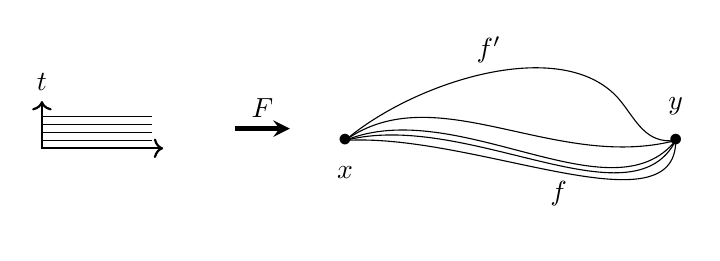
\begin{tikzpicture}[xscale=0.7, yscale=0.5]
        \draw [thick, <->] (1.5,6.2) node [above] {$t$} -- (1.5,5) -- (3.7,5);
        \draw (1.5,5.2) -- (3.5,5.2);
        \draw (1.5,5.4) -- (3.5,5.4);
        \draw (1.5,5.6) -- (3.5,5.6);
        \draw (1.5,5.8) -- (3.5,5.8);

        \draw [-stealth, ultra thick] (5, 5.5) -- (6,5.5) node[midway, above] {$F$};
        
        \coordinate (x) at (7, 5.2);
        \coordinate (y) at (13, 5.2);
        \node[label=below:$x$] (x) at (7, 5.2){$\bullet$};
        \node[label=above:$y$] (y) at (13, 5.2){$\bullet$};
        \draw (x.center) to [out=5, in=-90, edge node={node[below] {$f$}}] (y.center);
        \draw (x.center) to [out=20, in=-110] (y.center);
        \draw (x.center) to [out=30, in=-120] (y.center);
        \draw (x.center) to [out=45, in=-160] (y.center);
        \draw (x.center) to [out=50, in=-240, edge node={node[above] {$f'$}}] ++(5, 1) to [out=-60, in=-170] (y.center); 
    \end{tikzpicture}\end{center}
    空间$X$的基本广群$\Pi_1(X)$定义为如下范畴,其对象是$X$中的点,对任意$x,y \in X$,态射集$\Hom(x,y)$定义为所有从$x$到$y$的道路类;态射的合成定义为道路类的合成,而恒等态射$\identity_x$由静止道路$\forall t, \identity_x(t)=x$表示。对于给定的态射$f:x\rightarrow y$(同伦类中的某个代表元),其逆可以取为反向道路$f^{-1}:=f(1-t),t\in[0,1]$。

    可以验证这些操作都是良定的,并使得$\Pi_1(X)$成为广群。注意到$\Aut(X)=\Hom(x,x)$正好是以$x$为基点的\emph{基本群}$\pi_1(X,x)$.
\end{Exap}
    基本群是拓扑学中重要的不变量,它为每个空间$X$指定一个相应的代数结构(群)。 基本广群可以视为再高一阶的不变量:它为$X$指定一个范畴。但是应当注意还有大量拓扑信息被$\Pi_1(X)$的范畴结构遗漏了:除了道路的同伦类,还应该计入道路间的同伦等价,还可以设想同伦之间更有同伦,直至无穷。凡此种种都必须以更高阶的范畴语言反映。???

\begin{Def}[反范畴]任意范畴$\mathcal{C}$,其反范畴$\mathcal{C}^{\text{op}}$定义为:
    \begin{itemize}
        \item $\Obj(\mathcal{C}^{\text{op}})=\Obj(\mathcal{C})$
        \item $\forall X,Y \in \Obj(\mathcal{C}), \Hom_{\mathcal{C}^{\text{op}}}(X,Y):=\Hom_{\mathcal{C}}(Y,X)$
        \item $f \in \Hom_{\mathcal{C}^{\text{op}}}(Y,Z), g\in \Hom_{\mathcal{C}^{\text{op}}}(X,Y)$在$\mathcal{C}^{\text{op}}$中的合成$f \circ^{\text{op}}g$定义为$\mathcal{C}$中的反向合成$g\circ f$
        \item 恒等态射定义等同$\mathcal{C}$
    \end{itemize}
    容易验证$\mathcal{C}^{\text{op}}$满足范畴定义,且$(\mathcal{C}^{\text{op}})^{\text{op}}=\mathcal{C}$。
\end{Def}
    简而言之,$\mathcal{C}^{\text{op}}$的构造就是反转箭头,反转之后的范畴论公理依然成立,范畴论中的这种对称性也称作对偶原理。例如:$\mathcal{C}^{\text{op}}$中的单态射无非是$\mathcal{C}$中的满态射。

\section{函子与自然变换}

\begin{Def}[函子]设$\mathcal{C}',\mathcal{C}$为范畴。一个函子$F:\mathcal{C}'\rightarrow C$指:
    \begin{enumerate}
        \item 对象间的映射 $F:\Obj(\mathcal{C}')\rightarrow \Obj(\mathcal{C})$
        \item 态射间的映射 $F:\Mor(\mathcal{C}')\rightarrow \Mor(\mathcal{C})$ 使得
        \begin{itemize}
            \item $F$的来源和目标映射可交换$sF=Fs, tF=Ft$,等价的说法是$\forall X,Y\in \Obj(\mathcal{C}')$都有映射$F:\Hom_{\mathcal{C}'}(X,Y)\rightarrow \Hom_{\mathcal{C}}(FX,FY)$
            \item $F(g\circ f)=F(g)\circ F(f); F(\identity_X)=\identity_{FX}$
        \end{itemize}
    \end{enumerate}
    对于$F:\mathcal{C}_1\rightarrow \mathcal{C}_2, G:\mathcal{C}_2\rightarrow \mathcal{C}_3$,合成函子$G\circ F:\mathcal{C}_1\rightarrow \mathcal{C}_3$的定义是显然的:取合成映射
    \begin{gather*}
        \Obj(\mathcal{C}_1)\xrightarrow{F} \Obj(\mathcal{C}_2)\xrightarrow{G} \Obj(\mathcal{C}_3)       \\
        \Mor(\mathcal{C}_1)\xrightarrow{F} \Mor(\mathcal{C}_2)\xrightarrow{G}\Mor(\mathcal{C}_3)    \\
    \end{gather*}
\end{Def}
旧文献常将上述函子称为$\mathcal{C}'$到$\mathcal{C}$的共变函子,形如$F:(\mathcal{C}')^{\text{op}}\rightarrow \mathcal{C}$的函子为反变函子。

\begin{Rmk}
    从$\mathcal{C'}$到$\mathcal{C}$和从$(\mathcal{C}')^{\text{op}}$到$\mathcal{C}^{\text{op}}$的函子是一回事。为区分,对于函子$F:\mathcal{C}'\rightarrow \mathcal{C}$,反范畴间的相应函子记为$F^{\text{op}}:(\mathcal{C}')^{\text{op}}\rightarrow \mathcal{C}^{\text{op}}$
\end{Rmk}

\begin{Def}[函子的满性,忠实性,全性]
    对于函子$F:\mathcal{C}'\rightarrow \mathcal{C}$
    \begin{enumerate}
        \item 本质满的:若$\mathcal{C}$中任一对象都同构于某个$FX$
        \item 忠实的: 若$\forall X,Y\in \Obj(\mathcal{C}')$,映射$\Hom_{\mathcal{C}'}(X,Y)\rightarrow \Hom_{\mathcal{C}}(FX,FY)$都是单射
        \item 全的:上述映射对$\forall X,Y\in \Obj(\mathcal{C}')$都是满射
    \end{enumerate}
\end{Def}

\begin{Exap}[函子].
    \begin{enumerate}
        \item 子范畴$\mathcal{C}'\subset \mathcal{C}$给出一个包含函子$\iota:\mathcal{C}' \hookrightarrow \mathcal{C}$;包含函子总是忠实的,它是全函子当且仅当$\mathcal{C}'$是全子范畴。取$\mathcal{C}'=\mathcal{C}$就得到恒等函子$\identity_{\mathcal{C}}:\mathcal{C}\rightarrow \mathcal{C}$
        \item 考虑群范畴$\cate{Grp}$.$\forall$群$G$,总是可以忘掉$G$的群结构而视之为集合,群同态当然也可以视为集合间的映射,此程序给出\emph{忘却函子}$\cate{Grp}\rightarrow \cate{Set}$。类似地给出忘却其它结构的忘却函子
        $\cate{Top}\rightarrow \cate{Set}$(忘却空间的拓扑结构),$\cate{Vect}(\Bbbk)\rightarrow \cate{Ab}$(忘掉$\Bbbk$-向量空间$V$的纯量乘法,只看它的加法群$(V,+)$)等等。这类函子显然忠实而非全。
        \item 考虑域$\Bbbk$上的向量空间范畴$\cate{Vect}(\Bbbk)$。对于任意$\Bbbk$-向量空间$V$,定义其对偶空间
        \[
            V^{\vee}:=\Hom_{\Bbbk}(V,\Bbbk)=\{\Bbbk \text{-线性映射}V\rightarrow \Bbbk\}
        \]
        任一线性映射$f:V_1\rightarrow V_2$诱导对偶空间的反向映射
        \begin{gather*}
            f^{\vee}:V_{2}^{\vee}\rightarrow V_1^{\vee} \\
            [\lambda:V_2 \rightarrow \Bbbk] \mapsto \lambda \circ f
        \end{gather*}
        易见$D:V\mapsto V^{\vee}, f\mapsto f^{\vee}$定义了函子$D:\cate{Vect}(\Bbbk)^{\text{op}}\rightarrow \cate{Vect}(\Bbbk)$,可以验证$D$是忠实的。根据反函子的定义合成函子$DD^{\text{op}}: \cate{Vect}(\Bbbk)\rightarrow \cate{Vect}(\Bbbk)$

        将$D$限制于有限维向量空间,得到函子$D:\cate{Vect}_f(\Bbbk)^{\text{op}}\rightarrow \cate{Vect}_f(\Bbbk)$和$DD^{\text{op}}:\cate{Vect}_{f}(\Bbbk)\rightarrow \cate(Vect)_{f}(\Bbbk)$,分别称为对偶和双对偶函子。
        
        \item 对于任意群$G$,定义导出子群$G_{\text{der}}$为子集$\{xyx^{-1}:x,y\in G\}$生成的正规子群。商群$G/G_{\text{der}}$是交换群,称作$G$的Abel化。对于任意群同态$\varphi:G\rightarrow H$,从定义可以看出$\varphi(G_{\text{der}})\subset H_{\text{der}}$,因此$\varphi$诱导出交换群的同态$\bar{\varphi}:G/G_{\text{der}}\rightarrow H/H_{\text{der}}$。容易验证$G\mapsto G/G_{\text{der}}, \varphi \mapsto \bar{\varphi}$定义了Abel化函子$\cate{Grp}\rightarrow \cate{Ab}$。Abel化函子不是忠实函子。
        \item 对任意带点拓扑空间$(X,x)$指定基本群$\pi_1(X,x)$,给出了函子$\cate{Top}_{\bullet}\rightarrow \cate{Grp}$。代数拓扑学中还有许多例子,例如空间的同调群$X\mapsto H_n(X;Z)$给出了一族函子$H_n:\cate{Top}\rightarrow \cate{Ab}$,其中$n\in \mathbb{Z}_{\geq 0}$,上同调群给出函子$H^n:\cate{Top}^{\text{op}}\rightarrow \cate{Ab}$。
    \end{enumerate}
\end{Exap}

\begin{Def}[自然变换,或函子间的态射] 函子$F,G:\mathcal{C}'\rightarrow \mathcal{C}$之间的自然变换$\theta$是一族态射
    \[
        \theta_X \in \Hom_{\mathcal{C}}(FX,GX), X\in \Obj(\mathcal{C}')
    \]
    使得下图所有$\mathcal{C}'$中的态射交换
    \begin{center}\begin{tikzcd}
        FX \arrow[r, "\theta_X"] \ar[d, "Ff"'] & GX \arrow[d, "Gf"] \\
        FY \arrow[r, "\theta_Y"'] & GY .
    \end{tikzcd}\end{center}
    上述自然变换写作$\theta:F \to G$,或图解为
    \[\begin{tikzcd}
            \mathcal{C}' \arrow[bend left=50, r, "F", ""' name=U] \arrow[bend right=50, r, "G"', "" name=D] & \arrow[Rightarrow, to path=(U)--(D) \tikztonodes, "\theta"] \mathcal{C}
    \end{tikzcd}\]
    上述带有双箭头$\Rightarrow$的图表有时也被称为2-胞腔,一种兴许更有益的看法是设想$\theta $为从$F$到$G$的一个同伦。
\end{Def}
\begin{Cvs}.
    我们也将自然变换$\theta:F \to G$称为从函子$F$到$G$的态射。实用中经常会省略严格的范畴论框架,只说态射$\theta_X:FX\to GX$对于变元$X$是\emph{自然}的,\emph{典范}的,或称满足\emph{函子性}。实践中经常把自然同构直接写成等号$=$。
\end{Cvs}

    几种自然变换的操作,包括纵、横两种合成
    \begin{itemize}
        \item 纵合成: 考虑$\mathcal{C}'$到$\mathcal{C}$的三个函子间的态射$\theta:F\to G,\psi:G\to H$。纵合成$\psi \circ \theta :=\{\psi_X \circ \theta_X :X \in \Obj(\mathcal{C})\}$,图解:
        \[\begin{tikzcd}
            \mathcal{C}'
                \arrow[bend left=70, rr, "F", ""' name=U]
                \arrow[rr, "G" name=MM, ""' name = M]
                \arrow[bend right=70, rr, "" name=D, "H"'] & &
            \arrow[Rightarrow, to path=(U) -- (MM) \tikztonodes, "\theta"]
            \arrow[Rightarrow, to path=(M) -- (D) \tikztonodes, "\psi"]
            \mathcal{C}
        \end{tikzcd}
        \quad \text{合成为} \quad
        \begin{tikzcd}
            \mathcal{C}'
                \arrow[bend left = 50, rr, "F", ""' name = U]
                \arrow[bend right = 50, rr, "" name = D, "H"']  &&
            \arrow[Rightarrow, to path = (U) -- (D) \tikztonodes, "\psi \circ \theta"]
            \mathcal{C}
        \end{tikzcd}\]
        \item 横合成:考虑函子
        \begin{tikzcd}
            \mathcal{C}''
                \arrow[bend left = 30, r, "F_1"]
                \arrow[bend right = 30, r, "F_2"] &
            \mathcal{C}'
                \arrow[bend left = 30, r, "G_1"]
                \arrow[bend right = 30, r, "G_2"] &
            \mathcal{C}
        \end{tikzcd}
        及态射$\theta:F_1 \to F_2, \psi: G_1 \to G_2$。现定义横合成$\psi\circ \theta: G_1 \circ F_2 \to G_2 \circ F_2$。注意到对所有$X\in \Obj(\mathcal{C}'')$,根据$\psi$的自然性,图表
        \[\begin{tikzcd}
            G_1 F_1(X)
                \arrow[r, "{\psi_{F_1 X}}"]
                \arrow[d, "{G_1(\theta_X)}"'] &
            G_2 F_1(X)
                \arrow[d, "{G_2(\theta_X)}"]  \\
            G_1 F_2(X)
                \arrow[r, "{\psi_{F_2 X}}"'] &
            G_2 F_2(X)
        \end{tikzcd}\]
        交换。对角合成$\searrow$记作$(\psi \circ \theta)_X:G_1 F_1 (X) \to G_2 F_2 (X)$, 此即所求的横合成,我们马上会证明它的自然性。图解:
        \[\begin{tikzcd}
            \mathcal{C}''
                \arrow[bend left = 50, r, "F_1", ""' name = U1]
                \arrow[bend right = 50, r, "" name = D1,"F_2"'] &
            \mathcal{C}'
                \arrow[bend left = 50, r, "G_1", ""' name = U2]
                \arrow[bend right = 50, r, "" name = D2, "G_2"'] &
            \mathcal{C}
            \arrow[Rightarrow, to path = (U1) -- (D1) \tikztonodes, "\theta"]
            \arrow[Rightarrow, to path = (U2) -- (D2) \tikztonodes, "\psi"]
        \end{tikzcd}
        \quad \text{合成为} \quad
        \begin{tikzcd}
            \mathcal{C}''
                \arrow[bend left = 50, rr, "{G_1 F_1}", ""' name = U]
                \arrow[bend right = 50, rr, "" name = D, "{G_2 F_2}"'] & &
            \mathcal{C}
            \arrow[Rightarrow, to path = (U) -- (D) \tikztonodes, "{\psi \circ \theta}"]
        \end{tikzcd}\]
        \item 横合成的特例
        \[\begin{tikzcd}
            \mathcal{C}_1
                \arrow[r, "H"] &
            \mathcal{C}_2
                \arrow[bend left = 50, r, "F", ""' name = U]
                \arrow[bend right = 50, r, "" name = D, "G"'] &
            \mathcal{C}_3
                \arrow[r, "K"]  &
            \mathcal{C}_4
            \arrow[Rightarrow, to path = (U)--(D) \tikztonodes, "\theta"]
        \end{tikzcd}\]
        对左边三项:$\theta H:FH\to GH$简记横合成$\theta\circ\identity_{H}$;具体地说,$(\theta H)_X = \theta_{HX}:FH(X)\to GH(X)$;类似地处理右三项:$K\theta :KF\to KG$为横合成$\identity_{K}\circ \theta$,我们有$(K\theta)_X=K(\theta_X):KF(X)\to KG(X)$
    \end{itemize}

\Rmk{这里使用了同一个符号$\circ$表示纵横合成,如有混淆之虞将另作说明}

\begin{Lem}横纵合成$\{(\psi \circ \theta)_X\}_X$都是函子间的态射,而且各自满足严格结合律$(\phi \circ \psi) \circ \theta = \phi \circ (\psi \circ \theta)$。横纵合成之间满足关系:对于图表
    \[\begin{tikzcd}
        \mathcal{C}_1
            \arrow[bend left = 50, rr, ""' name = U1]
            \arrow[rr, "" name = UM1, ""' name = DM1]
            \arrow[bend right = 50, rr, "" name = D1]   & &
        \mathcal{C}_2
            \arrow[bend left = 50, rr, ""' name = U2]
            \arrow[rr, "" name = UM2, ""' name = DM2]
            \arrow[bend right = 50, rr, "" name = D2]  & &
        \mathcal{C}_3
        \arrow[Rightarrow, to path = (U1)--(UM1) \tikztonodes, "\theta"]
        \arrow[Rightarrow, to path = (DM1)--(D1) \tikztonodes, "\psi"]
        \arrow[Rightarrow, to path = (U2)--(UM2) \tikztonodes, "{\theta '}"]
        \arrow[Rightarrow, to path = (DM2)--(D2) \tikztonodes, "{\psi '}"]
    \end{tikzcd}\]
    以下的互换律成立
    \[
        \left( \psi' \underset{\text{纵}}{\circ} \theta ' \right)
        \underset{\text{横}}{\circ}
        \left( \psi  \underset{\text{纵}}{\circ} \theta   \right)
        =
        \left( \psi' \underset{\text{横}}{\circ} \psi \right)
        \underset{\text{纵}}{\circ}
        \left( \theta ' \underset{\text{横}}{\circ} \theta \right)
    \]
    \begin{proof} 证明横合成是函子间的态射。对于$\mathcal{C}''$中的态射$f:X\to Y$,图表
        \[\begin{tikzcd}
            G_1 F_1(X)
                \arrow[r, "G_1 \theta_X"]
                \arrow[d, "G_1 F_1 f"'] &
            G_1 F_2(X)
                \arrow[r, "\psi_{F_2 X}"]
                \arrow[d, "G_1 F_2 f"]  &
            G_2 F_2(X)
                \arrow[d, "G_2 F_2 f"] &    \\
            G_1 F_1(Y)
                \arrow[r, "G_1 \theta_Y"'] &
            G_1 F_2(Y)
                \arrow[r, "\psi_{F_2 Y}"'] &
            G_2 F_2(Y)
        \end{tikzcd}\]
        按定义,水平方向箭头合成后上下分别是$(\psi \circ \theta)_X$和$(\psi \circ \theta)_Y$。因为$\theta$ 是自然变换而$G_1$是函子,左方块交换;由于$\psi$是自然变换,右方块交换。将箭头分段作合成,可知整个大方块交换,此即$\psi\circ \theta$所需性质。

        现证明横合成的结合律:考虑函子间的态射
        \[\begin{tikzcd}
            \mathcal{C}'''
                \arrow[bend left = 50, r, "F_1", ""' name = U1]
                \arrow[bend right = 50, r, "" name = D1, "F_2"'] &
            \mathcal{C}''
                \arrow[bend left = 50, r, "G_1", ""' name = U2]
                \arrow[bend right = 50, r, "" name = D2, "G_2"'] &
            \mathcal{C}'
                \arrow[bend left = 50, r, "H_1", ""' name = U3]
                \arrow[bend right = 50, r, "" name = D3, "H_2"'] &
            \mathcal{C}
            \arrow[Rightarrow, to path = (U1)--(D1) \tikztonodes, "\theta"]
            \arrow[Rightarrow, to path = (U2)--(D2) \tikztonodes, "\psi"]
            \arrow[Rightarrow, to path = (U3)--(D3) \tikztonodes, "\phi"]
        \end{tikzcd}\]
        对任意$X\in \Obj(\mathcal{C}''')$考虑图表
        \[\begin{tikzcd}[row sep=small]
            & & H_1 G_2 F_2 (X)\arrow[rd] & \\
        H_1 G_1 F_1 (X)
            \arrow[r] &
        H1 G_2 F_1 (X)
            \arrow[ru]
            \arrow[rd] & &
        H_2 G_2 F_2 (X) \\
            & & H_2 G_2 F_1 (X)
                \arrow[ru] & 
        \end{tikzcd}\]
        $\psi$ 的自然性$G_2 F_1(X)\to G_2 F_2 (X)$可知菱形部分交换。按
        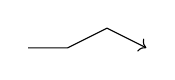
\begin{tikzpicture}[scale=0.5, baseline=(X)]
            \draw[->] (0,0)--(1,0)--(2,0.5)--(3,0);
            \coordinate (X) at (0,0);
        \end{tikzpicture}
        合成给出$(\phi \circ (\psi \circ \theta))_X$。按
        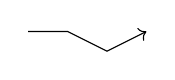
\begin{tikzpicture}[scale=0.5, baseline=(X)]
            \draw[->] (0,0)--(1,0)--(2,-0.5)--(3,0);
            \coordinate (X) at (0,-0.2);
        \end{tikzpicture}
        合成则给出$((\phi \circ \psi) \circ \theta)_X$。这里仍须用上交换图表,结合律证毕。

        最后一个等式可以同样按图索骥。
    \end{proof}
\end{Lem}
    任意函子$F$到自身有恒等态射$\identity_F:F\to F$。给定函子间的态射$\theta:F_1\to F_2$,若态射$\psi:F_2 \to F_1$满足$\psi \circ \theta=\identity_{F_1}, \theta \circ \psi = \identity_{F_2}$,则称$\psi$是$\theta$的逆。可逆的态射称为\emph{函子间的同构},写作$\theta:F_1 \xrightarrow{\sim} F_2$。由定义,若$\theta$的逆存在则唯一,记为$\theta^{-1}$,它无非是在范畴中“逐点地”取逆:$(\theta^{-1})_X:=(\theta_X)^{-1}:F_2X \xrightarrow{\sim}F_1X$。态射$\theta$可逆当且仅当每个$\theta_X$都可逆。易见同构的横纵合成仍是同构。函子间同构$\theta:F_1 \xrightarrow{\sim} F_2$的等价说法是称$\theta_X:F_1 X \xrightarrow{\sim}F_2 X$对变元$X$是\emph{自然同构}或\emph{典范同构}。

\begin{Def}[等价]如果一对函子
    \begin{tikzcd}
        \mathcal{C}_1
            \arrow[bend left = 20, r, "F"] &
        \mathcal{C}_2
            \arrow[bend left = 20, l, "G"]
    \end{tikzcd}
    满足性质:存在函子之间的同构$\theta:FG\xrightarrow{\sim}\identity_{\mathcal{C}_2}, \psi:GF\xrightarrow{\sim}\identity_{\mathcal{C}_1}$
    则称$G$是$F$的\emph{拟逆函子},并称$F$是范畴$\mathcal{C}_1$到$\mathcal{C}_2$的\emph{等价}。
    
    进一步,如果有$FG=\identity_{\mathcal{C}_2},GF=\identity_{\mathcal{C}_1}$,则称$F$是范畴间的\emph{同构},$G$是$F$的\emph{逆}。

    容易证明,等价的合成仍是等价。
\end{Def}
\section{函子范畴}
\section{泛性质}
\section{可表函子}
\section{伴随函子}
\section{极限}
\section{完备性}
\section{习题}
    %\chapter{幺半范畴}

\section{基本定义}
\section{严格性与融贯定理}
\section{辫结构}
\section{充实范畴}
\section{2-范畴一瞥}
\section{习题}

    %\section{Vector Spaces and Tensor Spaces}

\subsection{Vector Spaces}

\subsection{Dimensional Invariance}

\subsection{The Dual Vector Space}

\subsection{Linear Equations in a Skew Field}

\subsection{Linear Transformations}

\subsection{Tensors}

\subsection{Antisymmetric Multilinear Forms and Determinants}

\subsection{Tensor Products, Contraction, and Trace}
    %\chapter{环论初步}

\section{基本概念}
\section{几类特殊的环}
\section{交换环初探}
\section{间奏:${M\ddot{o}bius}$反演 }
\section{环的极限与完备化}
\section{从幺半群环刀多项式环}
\section{唯一分解性}
\section{对称多项式入门}
\section{习题}
    %\section{Theory of Fields}

\subsection{Subfields. Prime Fields}

\subsection{Adjunction}

\subsection{Simple Field Extensions}

\subsection{Finite Field Extensions}

\subsection{Algebraic Field Extensions}

\subsection{Roots of Unity}

\subsection{Galois Fields (Finite Commutative Fields)}

\subsection{Separable and Inseparable Extensions}

\subsection{Perfect and Imperfect Fields}

\subsection{Simplicity of Algebraic Extensions. Theorem on the Primitive Element}

\subsection{Norms and Traces}
    %\chapter{代数初步}

\section{交换环上的代数}
\section{整性,有限性和Frobenius定理}
\section{代数和张量积}
\section{分次代数}
\section{张量代数}
\section{对称代数和外代数}
\section{牛刀小试:Grassmann簇}
\section{行列式,迹,判别式}
\section{习题}
    %\chapter{域扩张}

\section{扩张的几种类型}
\section{代数闭包}
\section{分裂域和正规扩张}
\section{可分性}
\section{本原元素定理}
\section{域扩张中的范数与迹}
\section{纯不可分扩张}
\section{超越扩张}
\section{张量积的应用}
\section{习题}
    %\chapter{Galois理论}

\section{有限Galois对应}
\section{无限Galois对应}
\section{有限域}
\section{分圆域}
\section{正规基定理}
\section{Kummer理论}
\section{根式解判准}
\section{尺规作图问题}
\section{习题}
    %\chapter{域的值域}

\subsection{滤子}
\subsection{Krull赋值与完备化}
\subsection{域上的赋值}
\subsection{绝对值,局部域和整体域}
\subsection{个案研究:单位闭圆盘}
\subsection{一般扩域的赋值}
\subsection{代数扩域的赋值}
\subsection{完备域中求根}
\subsection{Witt向量}
\subsection{习题}
\end{document}